\begin{tikzpicture}[
		unit/.style={
				node distance=5cm,
			},
		label/.style={
				text width=3cm,
				text centered,
			},
		link/.style={
				draw=black,
				line width=0.60mm,
			},
	]
	\node (phone) [unit]{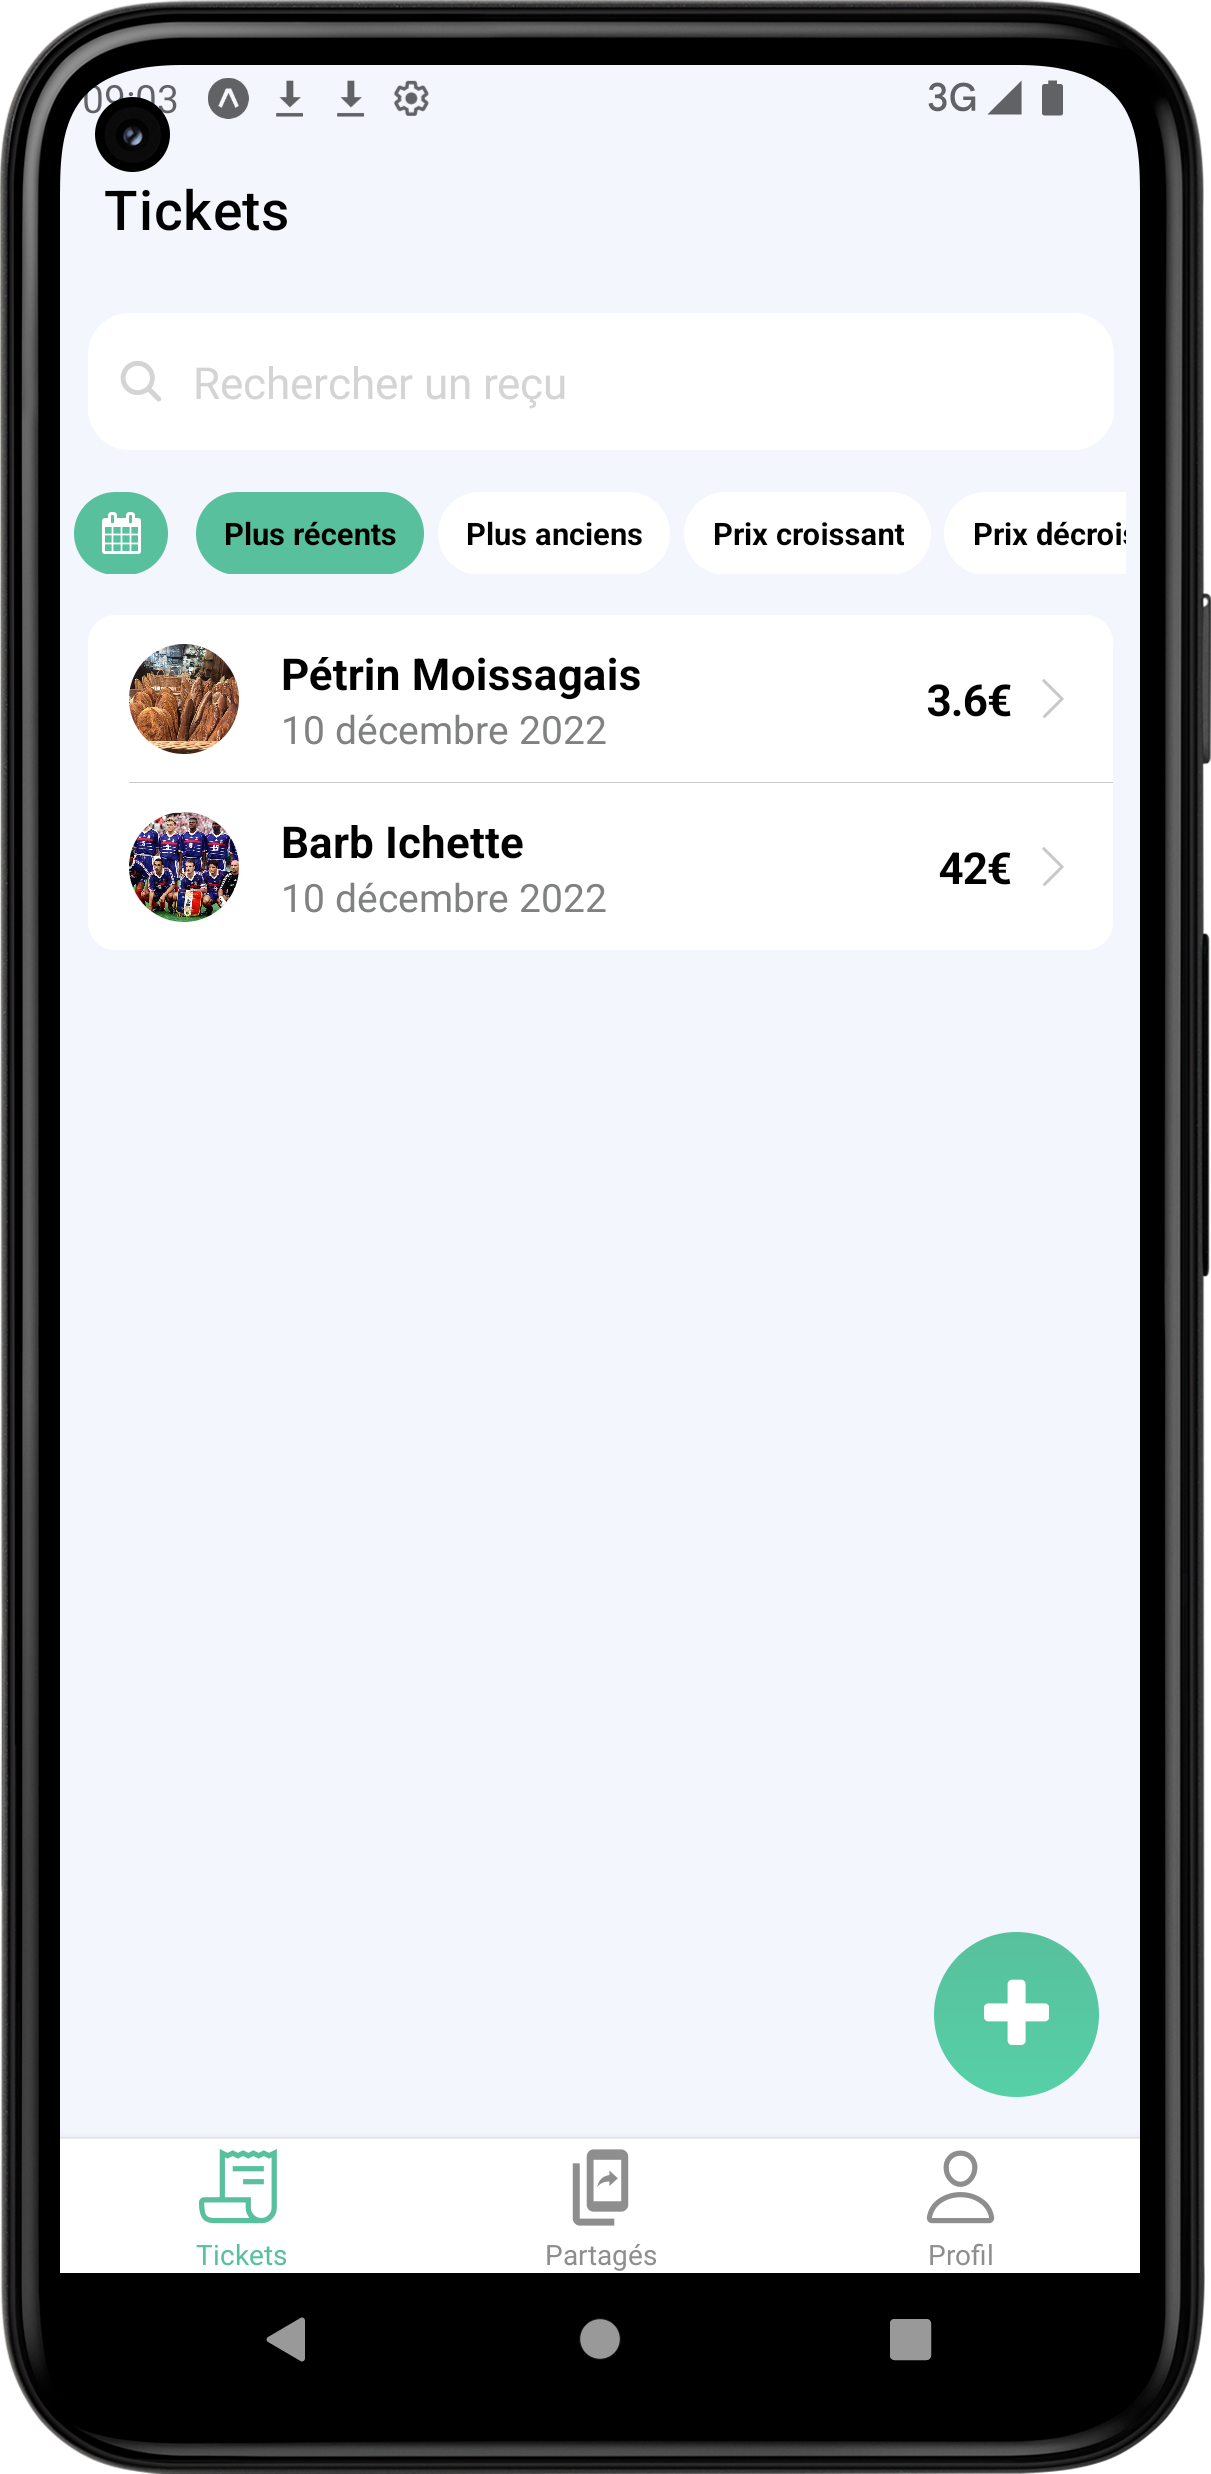
\includegraphics[width=.17\textwidth]{resources/mobile-app/view_receipts.png}};
	\node[below right] at (phone.south west) [label]{Application mobile client};

	\node (tpe) [left of=phone, unit]{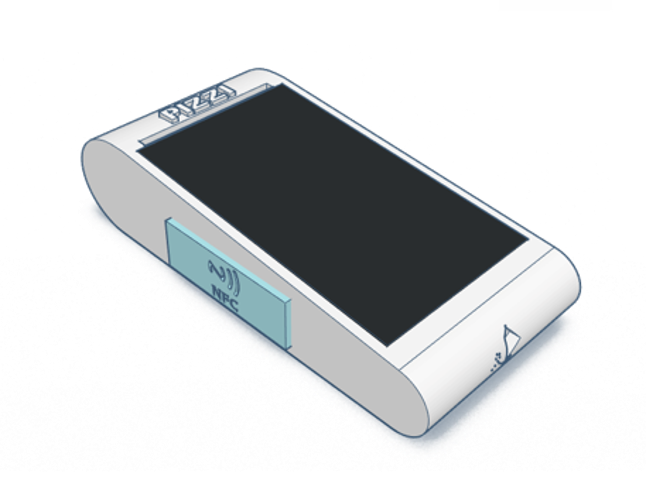
\includegraphics[width=.30\textwidth]{resources/tpe.png}};
	\node[below right] at (tpe.south west) [label]{Terminal de paiement connecté};

	\node (tablet) [left of=tpe, unit]{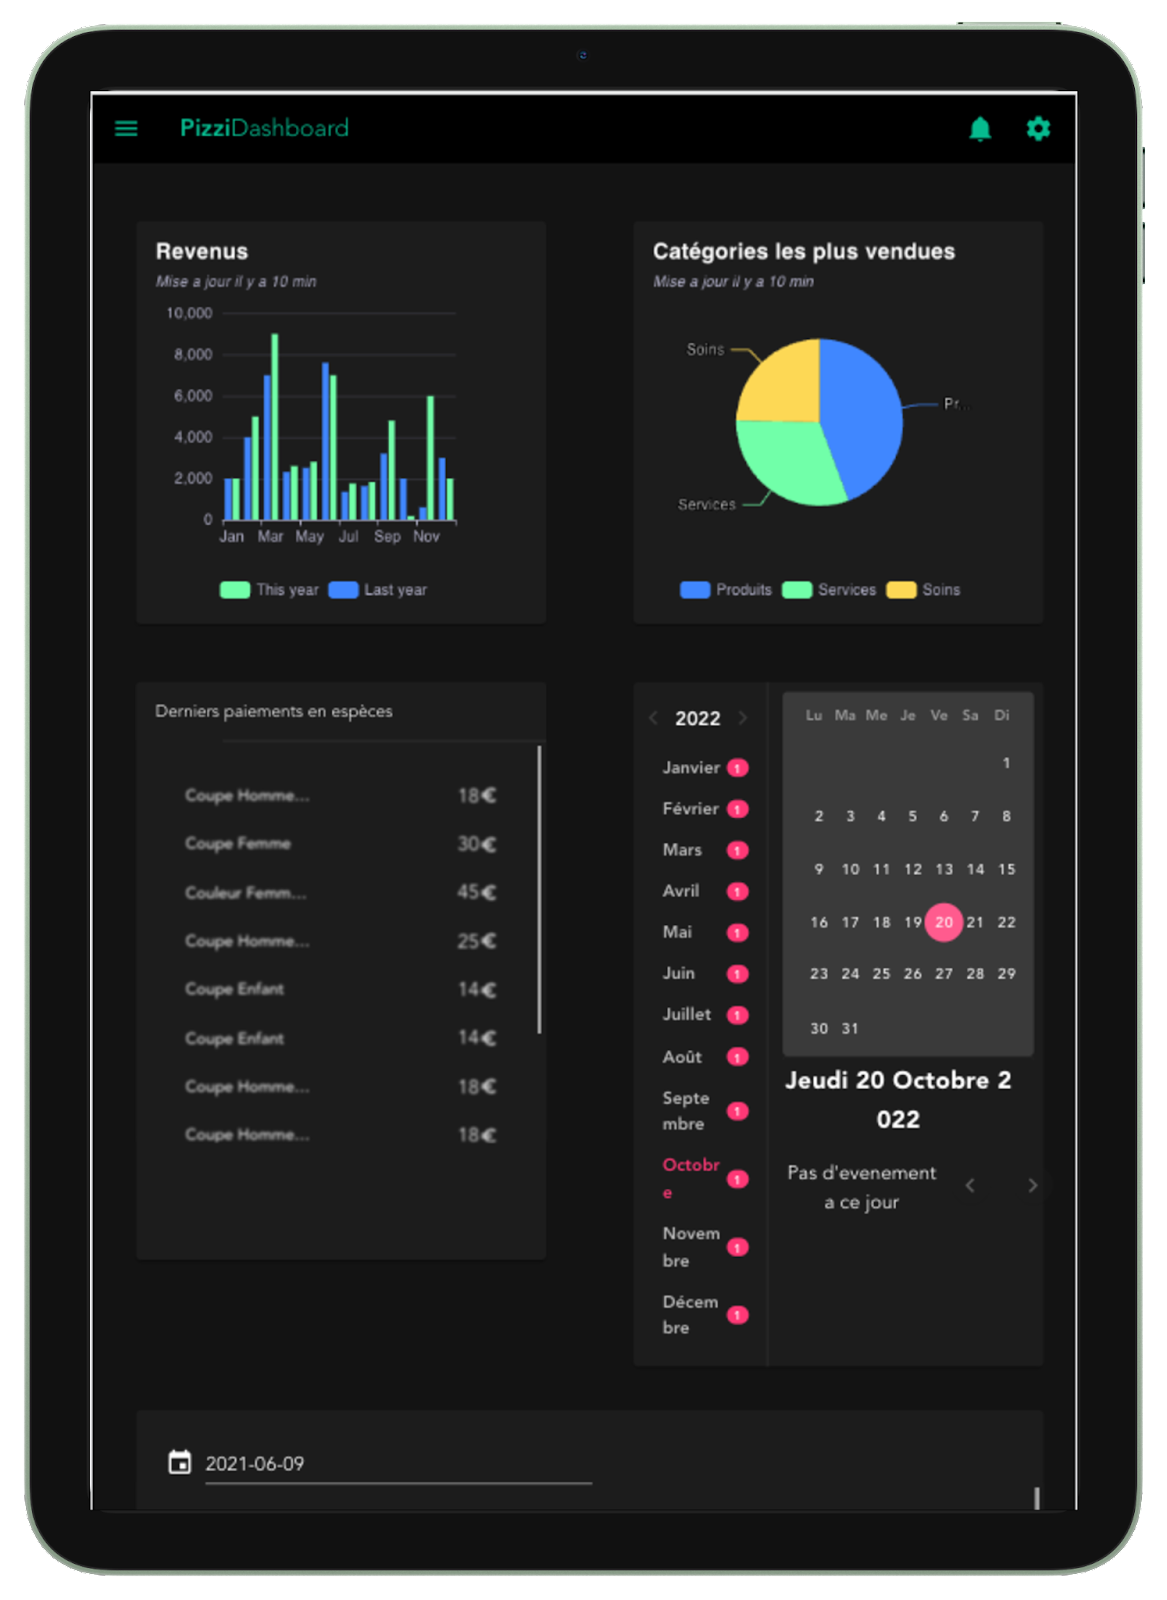
\includegraphics[width=.20\textwidth]{resources/shopkeeper-software/tablet.png}};
	\node[below right] at (tablet.south west) [label]{Logiciel commerçant};

	\draw [->, link] (tablet.east) -- (tpe.west) node[midway, fill=white] {1};
	\draw [->, link] ([yshift= 1ex] tpe.east) -- ([yshift= 1ex] phone.west) node[midway, fill=white] {2};
	\draw [->, link] ([yshift= -1ex] phone.west) -- ([yshift= -1ex] tpe.east) node[midway, fill=white] {3};
\end{tikzpicture}
